% !TeX root = ../dokumentation.tex

\addchap{\langanhang} 

{\Large
\begin{enumerate}[label=\Alph*.]
	\item Anleitung für Usability Testing
\end{enumerate}
}
\pagebreak
%\includepdf[pages=-,scale=.9,pagecommand={}]{Aufgabenstellung.pdf} % PDF um 10% verkleinert einbinden --> Kopf- und Fußzeile  werden so korrekt dargestellt. Die Option `pages' ermöglicht es, eine bestimmte Sequenz von Seiten (z.B. 2-10 oder `-' für alle Seiten) auszuwählen.
%\pagebreak
\section*{A. Anleitung für Usability Testing}
\label{apx:manual}
Die Applikation \textit{Machine Learning Training Data Generator} wird benutzt, um ein Modell zur Generierung von Daten zu erstellen und Daten daraus zu generieren.

\subsection*{Bedienung des Graph-Editors}

Das Modell wird dargestellt durch einen Graphen. Jeder Knoten in dem Graph entspricht einer Funktion die ausgeführt wird. Verbindungen (Kanten) übertragen Daten bzw. Zwischenergebnisse von einem Knoten zu einem anderen.

\begin{figure}[H]
    \centering
    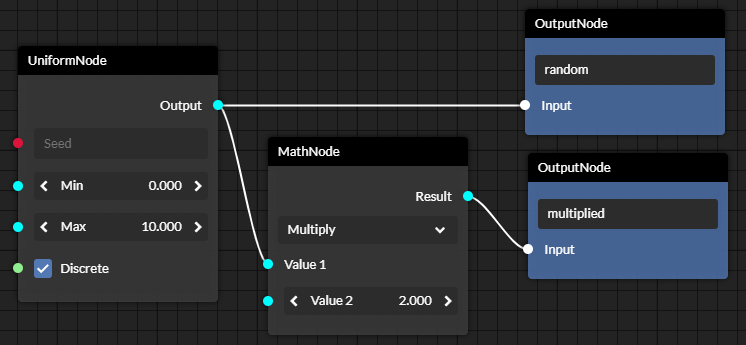
\includegraphics[width=1\textwidth]{simple_example.PNG}
\end{figure}

In diesem Beispiel ist ein einfaches Modell abgebildet. Es besteht aus einem Knoten, der gleichverteilte, ganzzahlige Werte zwischen 0 und 10 generiert, sowie einem Mathematikknoten, der diesen Wert mit der Zahl 2 multipliziert. Sowohl der Ausgang des Zufallsknotens, als auch der Ausgang des Mathematikknotens werden als Spalte in den generierten Daten ausgegeben.

Die Ausgabe dieses Beispiels sieht folgendermaßen aus:
\begin{table}[H]
    \centering
    \setlength\extrarowheight{-5pt}
    \begin{tabular}{ | c | c | }
        \hline
        random & multiplied \\
        \hline
        9 & 18 \\
        1 & 2 \\
        4 & 8 \\
        6 & 12 \\
        5 & 10 \\
        \hline
    \end{tabular}
\end{table}

Neue Knoten können mit einem Rechtsklick im Editor hinzugefügt werden. Folgende Knoten stehen zur Auswahl:

\begin{itemize}
    \item \textbf{Werteknoten} können benutzt werden, um den gleichen Wert an verschiedene andere Knoten weiterzugeben. Es gibt sie für die Datentypen \textit{Boolean}, \textit{Number} und \textit{String}. Zusätzlich gibt es den Index-Knoten. Dieser gibt den aktuellen Index innerhalb des Berechnungsprozesses aus. Wird ein Wert nur für einen Knoten verwendet, kann dieser in der Regel direkt an der Eingangsschnittstelle des entsprechenden Knotens eingestellt werden; ein Werteknoten muss dafür nicht verwendet werden.
    \item \textbf{Zufallsknoten}
    \begin{itemize}
        \item \textbf{Gleichverteilung} mit einstellbarem Minimum und Maximum
        \item \textbf{Normalverteilung} mit einstellbarem Mittelwert $\mu$ und Standardabweichung\nobreakspace $\sigma$
        \item \textbf{Exponentialverteilung} mit einstellbarem $\lambda$
        \item \textbf{Anpassbare Verteilung}: Bei diesem Knoten kann die Wahrscheinlichkeitsdichtefunktion über einen grafischen Editor eingestellt werden. Die Wahrscheinlichkeitsdichtefunktion kann sowohl diskret als auch kontinuierlich sein.
        \item \textbf{Prozentuale Abweichung}: Dieser Knoten nimmt einen Wert und addiert einen zufälligen Wert zwischen $\pm \, \, inputValue \cdot \frac{percentage}{100}$
    \end{itemize}
    \item \textbf{Berechnungsknoten}
    \begin{itemize}
        \item \textbf{Mathematik}: Der Mathematikknoten wendet eine einstellbare mathematische Funktion, wie zum Beispiel Addition, Division oder trigonometrische Funktionen auf ein oder zwei Eingabedaten an
        \item \textbf{Funktion}: Der Funktionsknoten kann benutzt werden, um eine beliebige Funktion in JavaScript zu implementieren. Alle Eingangswerte werden im \texttt{this} Objekt zur Verfügung gestellt. Der Code muss ein Objekt zurückgeben, welches die Namen der Ausgangsschnittstellen als Keys und die dazugehörigen Werte enthält.
        \item \textbf{Boolean}: Dieser Knoten vergleicht zwei numerische Werte und gibt das Resultat des Vergleichs aus.
    \end{itemize}
    \item \textbf{Bedingungsknoten}: Bedingungsknoten können genutzt werden, um sicherzustellen, dass Ausgabedaten bestimmte Bedingungen erfüllen. Wenn an der Eingangsschnittstelle der Wert \texttt{false} anliegt, wird der aktuelle Datenpunkt neu berechnet.
    \item \textbf{Ausgabeknoten}: Jeder Ausgabeknoten repräsentiert eine Spalte in den generierten Ausgabedaten. Der Name der Spalte kann im Textfeld des Ausgabeknotens gesetzt werden.
\end{itemize}

Knoten können gelöscht werden, indem sie markiert werden und die Taste \enquote{Entf} gedrückt wird. Alternativ können Knoten auch mit einem Rechtsklick auf den Namen des Knotens und dem anschließenden Auswählen von \textit{Delete} im Kontextmenü gelöscht werden.

Um eine neue Verbindung zwischen Knoten zu erstellen, kann mit der Maus eine Linie zwischen zwei Schnittstellen gezogen werden. Eine bestehende Verbindung kann entfernt werden, indem die linke Maustaste an der Zielschnittstelle gedrückt wird und die Maus bei gedrückter linker Maustaste von der Schnittstelle weggezogen wird.

\subsection*{Bedienung der Applikation}

In der Menüleiste am oberen Bildschirmrand können mehrere Aktionen ausgewählt werden: Laden und Speichern, Berechnen von Daten, Exportieren der berechneten Daten in eine CSV-Datei. Um Daten zu exportieren, müssen diese zuvor durch einen Klick auf \textit{Calculate} berechnet worden sein.

Zusätzlich kann in der Menüleiste zwischen mehreren Ansichten gewechselt werden:
\begin{itemize}
    \item \textbf{Editor}: Im Editor kann das Modell bearbeitet werden
    \item \textbf{Settings}: In der Ansicht können Einstellungen wie zum Beispiel die Anzahl der zu generierenden Daten eingestellt werden.
    \item \textbf{Preview Data}: In der Vorschau werden 20 aus dem Modell generierte Datensätze in tabellarischer Form angezeigt.
    \item \textbf{Visualisation}: Die Visualisierung kann benutzt werden, um zwei numerische Spalten der Daten in einem Streudiagramm anzuzeigen.
\end{itemize}